\documentclass[conference]{assets/latex/IEEEtran}
\IEEEoverridecommandlockouts

\usepackage{amsmath,amssymb,amsfonts}
\usepackage{algorithmic}
\usepackage{graphicx}
\usepackage{textcomp}
\usepackage{xcolor}
\usepackage[backend=biber,style=numeric]{biblatex}
\addbibresource{assets/latex/report.bib}
\renewcommand*{\bibfont}{\footnotesize}

\graphicspath{{assets/latex/}}

\begin{document}

\title{CS6524 Computer Vision Lab 4\\ Optical Flow and Kalman Filters}

\author{\IEEEauthorblockN{Cormac Shannon}
\IEEEauthorblockA{\textit{Immersive Software Engineering} \\
\textit{University of Limerick}\\
Limerick, Ireland}
\and
\IEEEauthorblockN{[TODO: name]}
\IEEEauthorblockA{\textit{Immersive Software Engineering} \\
\textit{University of Limerick}\\
Limerick, Ireland}
\and
\IEEEauthorblockN{[TODO: name]}
\IEEEauthorblockA{\textit{Immersive Software Engineering} \\
\textit{University of Limerick}\\
Limerick, Ireland}
}

\maketitle

\begin{abstract}
We track an object through an occlusion by combining pyramidal Lucas-Kanade optical flow with a constant-velocity Kalman filter. Keypoints are only searched for where the image changes, and the object is taken to be the largest spatial cluster of moving keypoints. Its centre is estimated with a weighted rolling average of keypoints pooled over the last ten frames. On the three provided videos and three of our own with real occluders, the filter carries the object across every occlusion and reacquires it, with a prediction error at reappearance of 21 to 352\,px. Every error but one falls within about three standard deviations of the filter's own predicted uncertainty, and almost all of the error comes from the constant-velocity assumption rather than from the measurements.
\end{abstract}

\section{Introduction}

The task is to follow a moving object, keep predicting its position while it is hidden, and compare that prediction with where it is when it comes back.

Three videos were provided (01 to 03: an orange, a pen and a potato passing behind a synthetic checkerboard). We recorded three more (04 to 06) in which an orange ping-pong ball rolls along a windowsill behind a laptop, a sheet of paper and a carpet tile, re-encoded to 1280$\times$720 at 30\,fps. These add a real occluder, a hand pushing the ball, and a bright window that flickers in the background.

\section{Methodology}

\subsection{Optical flow and object selection}

Keypoints are tracked with OpenCV's pyramidal Lucas-Kanade implementation~\cite{lucas1981,bouguet2000}, using a 21$\times$21 window and 3 pyramid levels so that the fastest motion in our videos (about 40\,px/frame in 05) stays within reach of the coarsest level. Each point is also tracked backwards, and any point that does not return to within 1\,px of where it started is dropped~\cite{kalal2010}. This removes most bad tracks on low-texture surfaces and along occluder edges.

New Shi-Tomasi corners~\cite{shi1994} are added every second frame (at most 200, quality level 0.01, minimum distance 7\,px). Our first version ran \texttt{goodFeaturesToTrack} over the whole frame, and in 06 the textured carpet tile used up the entire corner budget while the ball received none. Detection is therefore restricted to a motion mask: pixels whose grey level changes by more than 12 between frames, dilated by 15\,px so that the object's edges are included. The static background contributes nothing to the measurement, so nothing is lost by ignoring it.

Points moving faster than 1\,px/frame are grouped into connected clusters (points within roughly 80\,px of each other), and the largest cluster is taken to be the object. Fewer than ten points in that cluster means there is no measurement for the frame, which is exactly what happens behind the occluder. For our own videos a region of interest restricted to the windowsill keeps the hand out of the selection. An earlier, colour-based version of this step circled the hand in 06, a static carrot in 02 and the cutting board in 03 for most of each video, because skin and wood fall inside an orange hue range and are larger than the object; motion turned out to be a far more general cue than colour.

\subsection{What is tracked: a pooled centre}

We track the centre of the object. The obvious estimate, the median of the current frame's keypoints, is poor: corners sit wherever the object has contrast, usually one edge, and they appear and disappear from frame to frame. Against a colour-segmented reference this median was 25 to 43\,px from the true centre of the ball (Table~\ref{tab:centre}).

Instead, the object's keypoints from the last $K=10$ frames are kept, each frame's points are shifted forward by the object's displacement since that frame, and the centre is their weighted mean,
\begin{equation}
\mathbf{c}_t = \frac{\sum_{k=0}^{K-1}\sum_{i} w_k\,\bigl(\mathbf{p}_{i,t-k} + \sum_{j=t-k+1}^{t}\mathbf{v}_j\bigr)}{\sum_{k}\sum_{i} w_k}, \qquad w_k = 0.8^k,
\end{equation}
where $\mathbf{v}_j$ is the median keypoint flow in frame $j$. Points from different frames cover different parts of the object, and on a rolling object a tracked point circles the centre, so its shifted history averages out towards it. The pool is emptied whenever the object is not measured, because its displacement while hidden is unknown. Fig.~\ref{fig:centre} shows the pooled points and both estimates.

\begin{figure}[t]
\centerline{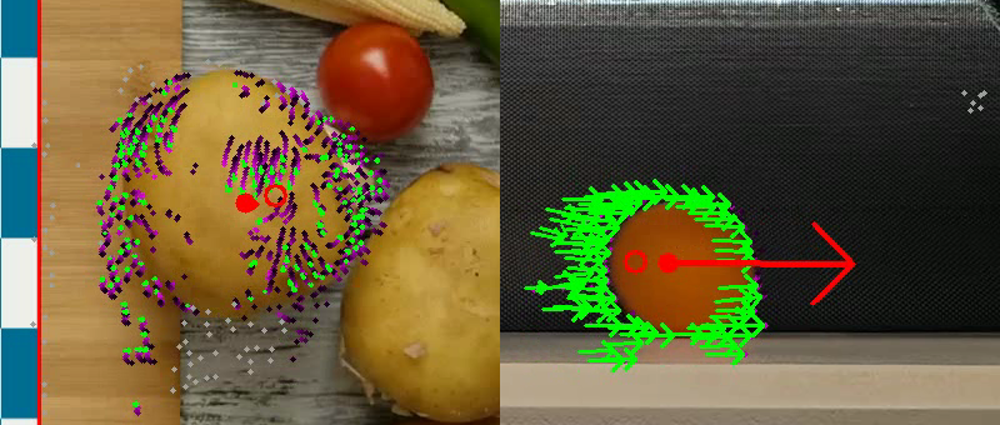
\includegraphics[width=\columnwidth]{fig_centre.png}}
\caption{Current object keypoints (green) and keypoints from the previous nine frames shifted to the current one (purple) for the potato in 03 (left) and the ball in 05 (right). The filled red dot is the pooled centre, the hollow circle the median of the current frame alone.}
\label{fig:centre}
\end{figure}

\subsection{Kalman filter}

The state is $\mathbf{x} = [x, y, v_x, v_y]^\top$ in pixels and pixels per frame, with a constant-velocity transition ($\Delta t = 1$ frame), using the notation of~\cite{becker}. We measure velocity as well as position, so $H = I_4$. The reason is visible in the data: the median keypoint flow has a frame-to-frame spread of about 1\,px/frame, while the measured position jumps by 10 to 40\,px as keypoints come and go. Discarding the most precise measurement we had would have made little sense. A position-only filter ($H = [I_2\;0]$, kept as an option) raised the error against the colour reference of Table~\ref{tab:centre} from 13.4 to 18.9\,px in 04 and from 14.3 to 39.3\,px in 05, and made no meaningful difference in 06 (44.6 against 43.6\,px).

Process noise follows the white-noise acceleration model~\cite{barshalom2001}: an unmodelled acceleration with standard deviation $\sigma_a = 0.5$\,px/frame$^2$ moves position by $a/2$ and velocity by $a$ in one frame, so per axis
\begin{equation}
Q = \sigma_a^2 \begin{bmatrix} 1/4 & 1/2 \\ 1/2 & 1 \end{bmatrix}.
\end{equation}
The ball in our videos slows by roughly 0.2\,px/frame$^2$ through friction, so 0.5 leaves room for pushes and bumps. Raising it to 1 or 2 increased the error in all three ball videos.

The measurement noise $R$ is diagonal and recomputed every frame from the optical flow itself, as the lab notes suggest. For velocity it is the spread of the keypoint flow. For position it took three attempts to get right, which we return to in Section~\ref{sec:discussion}. The final version treats each pooled frame as a roughly independent view of the object, dividing the keypoint spread by the square root of the effective number of pooled frames $\sum_k w_k$. Once ten frames of history exist it is never allowed below the centre's own residual noise, measured from how far $\mathbf{c}_t$ departs from $\mathbf{c}_{t-1} + \mathbf{v}_t$. $P_0$ is the first measurement's spread plus a margin of 10\,px and 5\,px/frame.

Three safeguards sit around the filter. A measurement is rejected if its squared Mahalanobis distance to the prediction exceeds the 99.9\% $\chi^2$ quantile. The track only starts after three consecutive frames of steady motion above 5\,px/frame, because hand jitter in 05 otherwise started it on the wrong thing. If three rejected measurements in a row agree with each other, the filter is re-initialised from them, which is how it recovers when the potato in 03 hits the other potatoes and stops dead.

\subsection{Occlusion and split trajectories}

The occlusion is the longest run of frames without an accepted measurement that ends with the object measured again. At that frame the trajectory is split in two. The real one continues with corrections. The ghost, the trajectory the filter would have followed had the object never returned, takes the filter's prediction for the reappearance frame (which uses nothing seen after the object disappeared) and keeps propagating it, along with its covariance, without any corrections. The prediction error is the distance between that prediction and the first measurement after reappearance, also expressed in standard deviations of the predicted position.

\begin{figure}[t]
\centerline{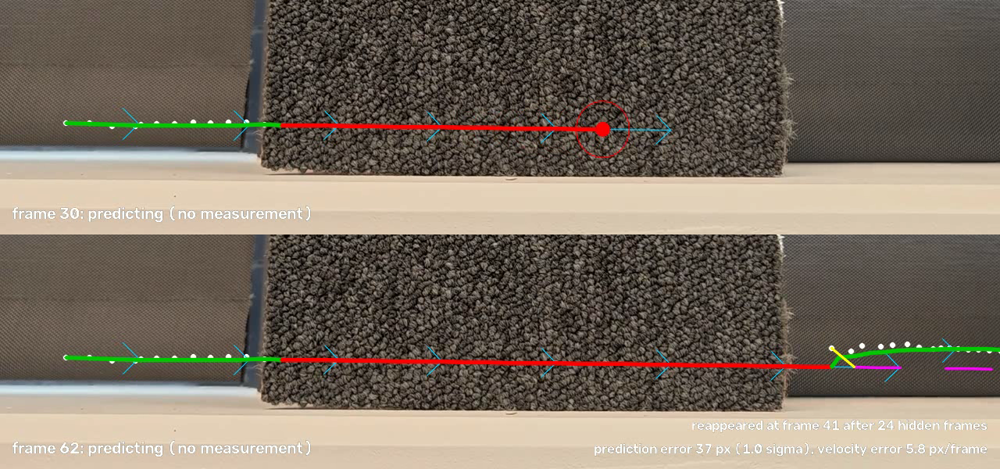
\includegraphics[width=\columnwidth]{fig_tracking.png}}
\caption{Video 06. Top: frame 30, the ball is behind the tile and the filter predicts (red) with a growing 2$\sigma$ ellipse. Bottom: frame 62, after the ball has reappeared and left the frame, with the prediction error at reappearance (yellow), the corrected track (green) and the ghost that ignores the ball's return (magenta). White dots are measurements, cyan arrows velocity every 5 frames.}
\label{fig:tracking}
\end{figure}

\section{Results}

All six videos produce a continuous track through the occlusion (Fig.~\ref{fig:tracking}) and every object is reacquired (Table~\ref{tab:reappear}). Table~\ref{tab:centre} compares the centre estimates with a colour-segmented reference, which was only reliable for the orange ball and only used on frames where the whole ball is in view.

\begin{table}[t]
\caption{Prediction at reappearance}
\begin{center}
\begin{tabular}{|c|c|c|c|c|}
\hline
\textbf{Video} & \textbf{Hidden} & \textbf{Position} & \textbf{In $\sigma$} & \textbf{Velocity} \\
 & \textbf{frames} & \textbf{error (px)} & & \textbf{error (px/f)} \\
\hline
01 & 33 & 318 & 4.3 & 5.0 \\
02 & 83 & 255 & 1.1 & 2.1 \\
03 & 19 & 118 & 2.8 & 2.4 \\
04 & 39 & 352 & 3.1 & 13.4 \\
05 & 15 & 21 & 0.9 & 6.5 \\
06 & 24 & 37 & 1.0 & 5.8 \\
\hline
\end{tabular}
\label{tab:reappear}
\end{center}
\end{table}

\begin{table}[t]
\caption{Mean distance to the colour-segmented centre (px)}
\begin{center}
\begin{tabular}{|c|c|c|c|c|}
\hline
 & \multicolumn{2}{|c|}{\textbf{Measured}} & \multicolumn{2}{|c|}{\textbf{Kalman}} \\
\cline{2-5}
\textbf{Video} & \textbf{median} & \textbf{pooled} & \textbf{median} & \textbf{pooled} \\
\hline
04 (7 frames) & 25.2 & 13.6 & 23.6 & 13.4 \\
05 (18 frames) & 42.9 & 22.7 & 19.3 & 14.3 \\
06 (14 frames) & 42.5 & 29.6 & 52.9 & 44.6 \\
\hline
\end{tabular}
\label{tab:centre}
\end{center}
\end{table}

\section{Discussion and failure analysis}
\label{sec:discussion}

\textbf{The filter leans on velocity.} Fig.~\ref{fig:gain} shows what happens inside the filter in 06. While the ball is visible the position gain mostly stays between 0.07 and 0.3, so the filter mostly integrates the precise velocity and only nudges its position towards the measurement. Behind the occluder no correction happens and $\sigma_x$ grows from 4\,px to 36\,px over 24 frames. The acceleration model makes the position variance grow with $t^3$, so $\sigma_x$ grows roughly as $t^{3/2}$, which is the upward curve in the grey region. When the ball reappears the gain jumps back to 0.6 and the filter takes most of the first measurement at face value.

\begin{figure}[t]
\centerline{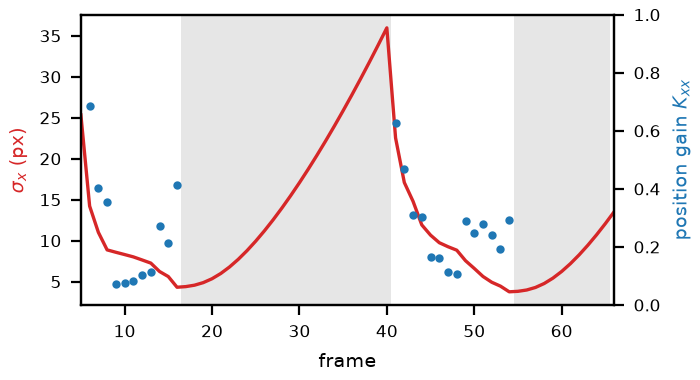
\includegraphics[width=\columnwidth]{fig_gain.png}}
\caption{Predicted position uncertainty $\sigma_x$ and position gain $K_{xx}$ in video 06. Grey: frames with no accepted measurement.}
\label{fig:gain}
\end{figure}

\textbf{Measurement noise was the hardest part to get right.} Our first $R$ divided the keypoint spread by $\sqrt{n}$, as if every keypoint carried independent error. The filter became about five times too confident in position, and its own gate rejected most of the real measurements (143 of 185 in 01, 100 of 113 in 03). The errors are not independent: they depend on which part of the object happens to have corners, so they are shared by all keypoints in a frame. Using the plain spread fixed the rejections but, once the pooled centre was introduced, kept the gain so low that the filter never shed the bias of its first few measurements; in 06 it stayed close to 50\,px ahead of the reference while its input had converged to within 7\,px. Estimating the centre's noise from only three residuals failed the other way, giving 1\,px and a filter that locked onto a centre that was still 55\,px off. The final rule gave the lowest or equal-lowest filter error of the three on every ball video, and improved on the original median measurement in each (Table~\ref{tab:centre}).

\textbf{The constant-velocity model explains most of the error.} The errors in Table~\ref{tab:reappear} are large in pixels but mostly modest in standard deviations, which means the filter's uncertainty was honest and the gate let every object back in. The large ones have physical causes the model cannot represent. In 04 the ball slowed from 31 to 18\,px/frame while hidden behind the laptop, giving a 352\,px overshoot. In 01 the orange speeds up while hidden: it covers about 650\,px in 31 frames, against the 12 to 14\,px/frame measured just before the occluder, and this is the one error well outside 3$\sigma$. In 02 the pen roughly doubles its speed behind the occluder, from about 2 to 4\,px/frame, and over 83 hidden frames that accumulates to 255\,px. Rolling also biases the velocity measurement itself: the top of a rolling ball moves at twice the speed of its centre, and early in 01, when the only keypoints were on top of the orange, the measured speed briefly reached 24\,px/frame before settling at about 14.

\textbf{Pooling cannot see what was never visible.} When an object enters the frame or comes out from behind the occluder, only its leading half is visible, and the pooled centre is biased forwards by 30 to 55\,px until the rest appears. This accounts for most of the remaining error in 06 (Table~\ref{tab:centre}), where the ball is only fully visible for about eight frames on either side of the tile.

\textbf{Threats to validity.} The colour reference only exists for the ball, covers between 7 and 18 frames per video, and its own centroid is imperfect. Videos 02 and 04 to 06 use small per-video settings (a lower start speed for the slow pen and a region of interest that excludes the hand), so the pipeline is not entirely free of tuning.

\textbf{With more time} we would add a deceleration term to the state, or run a small bank of motion models, to address the overshoot in 04 and the stop in 03. The centre could be estimated by fitting the object's outline to the pooled keypoints, which would remove the leading-edge bias, and corrections could be down-weighted until the pool holds enough frames to be trusted.

\section{Conclusion}

Restricting corner detection to moving regions, choosing the largest moving cluster and pooling keypoints over time gave a reliable, reasonably central measurement without any knowledge of the object's colour or shape. The filter carried all six objects through their occlusions with errors consistent with its own uncertainty. What limits the prediction is the motion model, not the measurement: objects that slow down, speed up or stop while hidden end up hundreds of pixels from where a constant-velocity filter expects them.

\printbibliography

\end{document}
